\let\negmedspace\undefined
\let\negthickspace\undefined
\documentclass[journal]{IEEEtran}
\usepackage[a5paper, margin=10mm, onecolumn]{geometry}
\usepackage{lmodern} % Ensure lmodern is loaded for pdflatex
\usepackage{tfrupee} % Include tfrupee package

\setlength{\headheight}{1cm} % Set the height of the header box
\setlength{\headsep}{0mm}     % Set the distance between the header box and the top of the text

\usepackage{gvv-book}
\usepackage{gvv}
\usepackage{cite}
\usepackage{amsmath,amssymb,amsfonts,amsthm}
\usepackage{algorithmic}
\usepackage{graphicx}
\usepackage{textcomp}
\usepackage{xcolor}
\usepackage{txfonts}
\usepackage{listings}
\usepackage{enumitem}
\usepackage{mathtools}
\usepackage{gensymb}
\usepackage{comment}
\usepackage[breaklinks=true]{hyperref}
\usepackage{tkz-euclide} 
\usepackage{listings}
\def\inputGnumericTable{}                                 
\usepackage[latin1]{inputenc}                                
\usepackage{color}                                            
\usepackage{array}                                            
\usepackage{longtable}                                       
\usepackage{calc}                                             
\usepackage{multirow}                                         
\usepackage{hhline}                                           
\usepackage{ifthen}                                           
\usepackage{lscape}

\begin{document}
	
	\bibliographystyle{IEEEtran}
	\vspace{3cm}
	
	\title{10.3.3.2}
	\author{EE24BTECH11047 - Niketh Prakash Achanta}
	% \maketitle
	% \newpage
	% \bigskip
	{\let\newpage\relax\maketitle}
	
	\renewcommand{\thefigure}{\theenumi}
	\renewcommand{\thetable}{\theenumi}
	\setlength{\intextsep}{10pt} % Space between text and floats
	
\textbf{Question:} Solve the system of equations
\begin{align*}
2x + 3y &= 11 \\
2x - 4y &= -24
\end{align*}
and hence find the value of \( m \) for which
\begin{align*}
y &= mx + 3
\end{align*}

\textbf{Solution}\\
\textbf{Theoretical solution:}\\
\textbf{Step 1: Solving the system of equations}

We can use the elimination method. First, subtract equation (2) from equation (1) to eliminate \( x \):
\begin{align}
(2x + 3y) - (2x - 4y) &= 11 - (-24) \\
2x + 3y - 2x + 4y &= 11 + 24 \\
7y &= 35 \\
y &= 5
\end{align}

\textbf{Step 2: Substituting \( y = 5 \) into one of the original equations}

Substitute \( y = 5 \) into equation (1):
\begin{align}
2x + 3(5) &= 11 \\
2x + 15 &= 11 \\
2x &= 11 - 15 \\
2x &= -4 \\
x &= -2
\end{align}

Thus, the solution to the system of equations is \( x = -2 \) and \( y = 5 \).

\textbf{Step 3: Finding the value of \( m \) for the equation \( y = mx + 3 \)}

We are given the equation \( y = mx + 3 \). Since we know that \( y = 5 \) when \( x = -2 \), substitute these values into the equation:
\begin{align}
5 &= m(-2) + 3 \\
5 &= -2m + 3 \\
5 - 3 &= -2m \\
2 &= -2m \\
m &= -1
\end{align}

Thus, the value of \( m \) is \( \boxed{-1} \).

	\textbf{Computational Solution:}
	\newline
\section*{Solution using LU Factorization}

Given the system of linear equations:
\begin{align}
2x + 3y &= 11, \label{eq1} \\
2x - 4y &= -24. \label{eq2}
\end{align}

We rewrite the equations as:
\begin{align}
x_1 &= x, \\
x_2 &= y,
\end{align}
giving the system:
\begin{align}
2x_1 + 3x_2 &= 11, \label{eq3} \\
2x_1 - 4x_2 &= -24. \label{eq4}
\end{align}

\subsection*{Step 1: Convert to Matrix Form}
We write the system as:
\begin{align}
A \mathbf{x} &= \mathbf{b},
\end{align}
where:
\begin{align}
A &= \begin{bmatrix} 2 & 3 \\ 2 & -4 \end{bmatrix}, \\
\mathbf{x} &= \begin{bmatrix} x_1 \\ x_2 \end{bmatrix}, \\
\mathbf{b} &= \begin{bmatrix} 11 \\ -24 \end{bmatrix}.
\end{align}

\subsection*{Step 2: LU factorization using update equations}
Given a matrix $ \mathbf{A} $ of size $ n \times n $, LU decomposition is performed row by row and column by column. The update equations are as follows:\\
\textbf{Step-by-Step Procedure:}\\
1. Initialization: 
- Start by initializing $ \mathbf{L} $ as the identity matrix $ \mathbf{L} = \mathbf{I} $ and $ \mathbf{U} $ as a copy of $ \mathbf{A} $.
	
2. Iterative Update:
- For each pivot $ k = 1, 2, \ldots, n $:
- Compute the entries of $ U $ using the first update equation.
- Compute the entries of $ L $ using the second update equation.
	
3. Result:
- After completing the iterations, the matrix $ \mathbf{A} $ is decomposed into $ \mathbf{L} \cdot \mathbf{U} $, where $ \mathbf{L} $ is a lower triangular matrix with ones on the diagonal, and $ \mathbf{U} $ is an upper triangular matrix.
	
\subsection*{1. Update for $ U_{k,j} $ (Entries of $ U $)}

For each column $ j \geq k $, the entries of $ U $ in the $ k $-th row are updated as:
\begin{align}
U_{k,j} &= A_{k,j} - \sum_{m=1}^{k-1} L_{k,m} \cdot U_{m,j}, \quad \text{for } j \geq k.
\end{align}
This equation computes the elements of the upper triangular matrix $ \mathbf{U} $ by eliminating the lower triangular portion of the matrix.

\subsection*{2. Update for $ L_{i,k} $ (Entries of $ L $)}

For each row $ i > k $, the entries of $ L $ in the $ k $-th column are updated as:
\begin{align}
L_{i,k} &= \frac{1}{U_{k,k}} \left( A_{i,k} - \sum_{m=1}^{k-1} L_{i,m} \cdot U_{m,k} \right), \quad \text{for } i > k.
\end{align}
This equation computes the elements of the lower triangular matrix $ \mathbf{L} $, where each entry in the column is determined by the values in the rows above it.\\

\subsection*{Step 2: LU Factorization of Matrix A}
We decompose $A$ as:
\begin{align}
A &= LU,
\end{align}
where $L$ is a lower triangular matrix and $U$ is an upper triangular matrix.
By running the iteration code, we get the $L$ and $U$ matrices:
\begin{align}
L &= \begin{bmatrix} 1 & 0 \\ 1 & 1 \end{bmatrix}, \\
U &= \begin{bmatrix} 2 & 3 \\ 0 & -7 \end{bmatrix}.
\end{align}

\subsection*{Step 3: Solve $L\mathbf{y} = \mathbf{b}$ (Forward Substitution)}
We solve:
\begin{align}
L\mathbf{y} = \mathbf{b} \quad \text{or} \quad \begin{bmatrix} 1 & 0 \\ 1 & 1 \end{bmatrix} \begin{bmatrix} y_1 \\ y_2 \end{bmatrix} = \begin{bmatrix} 11 \\ -24 \end{bmatrix}.
\end{align}
From the first row:
\begin{align}
y_1 &= 11.
\end{align}
From the second row:
\begin{align}
y_1 + y_2 &= -24 \quad \implies \quad 11 + y_2 = -24 \quad \implies \quad y_2 = -35.
\end{align}

Thus:
\begin{align}
\mathbf{y} &= \begin{bmatrix} 11 \\ -35 \end{bmatrix}.
\end{align}

\subsection*{Step 4: Solve $U\mathbf{x} = \mathbf{y}$ (Backward Substitution)}
We solve:
\begin{align}
U\mathbf{x} = \mathbf{y} \quad \text{or} \quad \begin{bmatrix} 2 & 3 \\ 0 & -7 \end{bmatrix} \begin{bmatrix} x_1 \\ x_2 \end{bmatrix} = \begin{bmatrix} 11 \\ -35 \end{bmatrix}.
\end{align}
From the second row:
\begin{align}
-7x_2 &= -35 \quad \implies \quad x_2 = 5.
\end{align}
From the first row:
\begin{align}
2x_1 + 3x_2 &= 11 \quad \implies \quad 2x_1 + 3(5) = 11, \\
2x_1 + 15 &= 11 \quad \implies \quad 2x_1 = -4, \\
x_1 &= -2.
\end{align}

Thus:
\begin{align}
\mathbf{x} &= \begin{bmatrix} x_1 \\ x_2 \end{bmatrix} = \begin{bmatrix} -2 \\ 5 \end{bmatrix}.
\end{align}

\subsection*{Final Solution}
The solution is:
\begin{align}
x &= -2, \\
y &= 5.
\end{align}
\subsection*{Step 5: Finding the Value of \( m \)}

We are given the equation \( y = mx + 3 \), and we know that \( x = -2 \) and \( y = 5 \) from the solution of the system. Substituting these values into the equation:
\begin{align}
5 &= m(-2) + 3.
\end{align}
Solving for \( m \):
\begin{align}
5 - 3 &= -2m, \\
2 &= -2m, \\
m &= -1.
\end{align}

Thus, the value of \( m \) is \( \boxed{-1} \).

\subsection*{Final Solution}
The solution is:
\begin{align}
x &= -2, \\
y &= 5, \\
m &= -1.
\end{align}
	\begin{figure}[!ht]
		\centering
		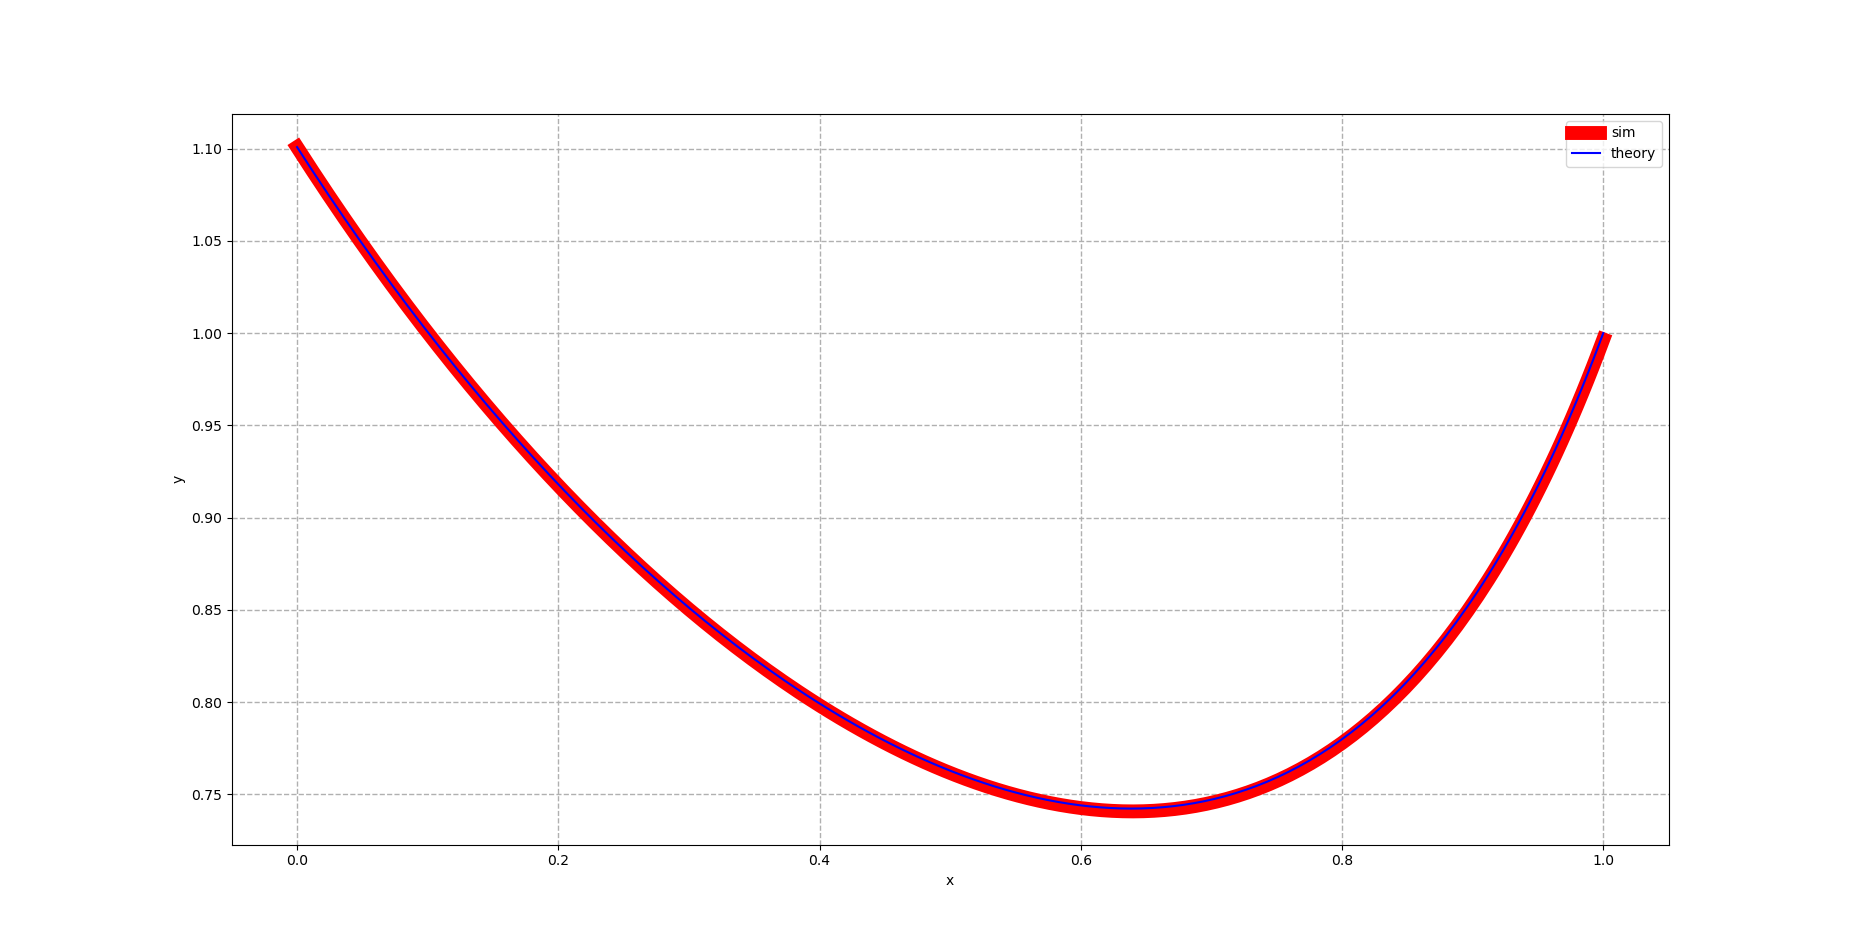
\includegraphics[width=\columnwidth]{/home/niketh/EE1003/3.3.2/figs/Figure_1.png}
		\caption{}
	\end{figure}
\end{document}
